


%%%%%%%%%%%%%%%%%%%%%%%%%%%%%%%%%%%%%%%%%%%%%%%%%%%%%%%%%%%%%%%%%%%%%%%%
\section{Agentes Racionais}
\begin{frame}

    \frametitle{Características aos SMAs}
    \begin{itemize}
    \pause
      \item 
\pause
      \item cap 2
    
    \end{itemize}
\end{frame}

\subsection{Tipos de Agentes}
\begin{frame}

Os agentes podem ser de dois tipos:
\begin{description}

 \item[Agentes Reativos (ou reflexivos):] geralmente são agentes simples, escolhem suas ações baseados exclusivamente nas percepções que têm do ambiente. Normalmente possui representação do conhecimento implícito  no código, por não  possuirem
  memória, não tem histórico dos fatos  e das ações que executou.

  \item[Agentes Cognitivos:]  têm uma representação simbólica explícita do seu ambiente, no qual eles podem argumentar e predizer eventos futuros. São dirigidos por intenções, isto é, por metas explícitas que conduzem seu comportamento e os tornam capazes de escolher entre possíveis ações. 
  Engloba as características: percepção, ação, comunicação, representação, 
  motivação, deliberação, raciocínio e aprendizagem. 

\end{description}

\end{frame}


\subsection{Agentes Racionais}

\begin{frame}

  \frametitle{Agente em seu ambiente}
    
\begin{figure}[!ht]
  \centering
  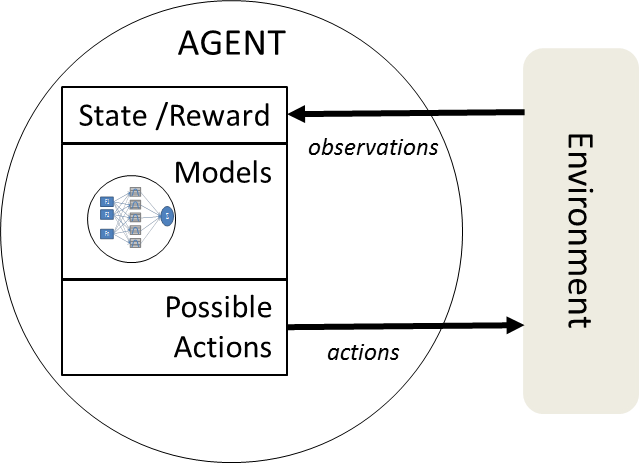
\includegraphics[height =.6\textheight,width=.7\textwidth]{figuras/agente_ambiente_ciclo.png}
  \caption{Ciclo do agente}
%\label{ag_01}
\end{figure}
    
\end{frame}



\begin{frame}

  \frametitle{Arquitetura clássica de um agente reflexivo}
    
\begin{figure}[!ht]
\centering
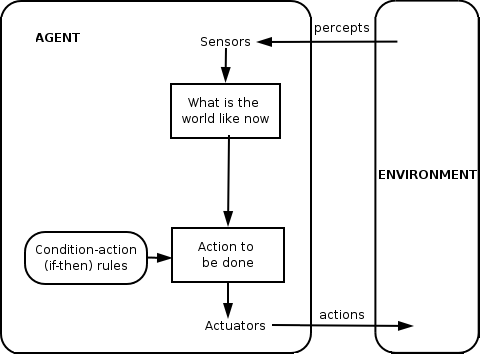
\includegraphics[width=.6\textwidth]{figuras/agent-reflexivo.png}
\caption{Arquitetura clássica}
\label{ag_01}
\end{figure}
    
\end{frame}


\begin{frame}

  \frametitle{Arquitetura clássica de um agente que \textit{aprende} -- desejável}
    
\begin{figure}[!ht]
\centering
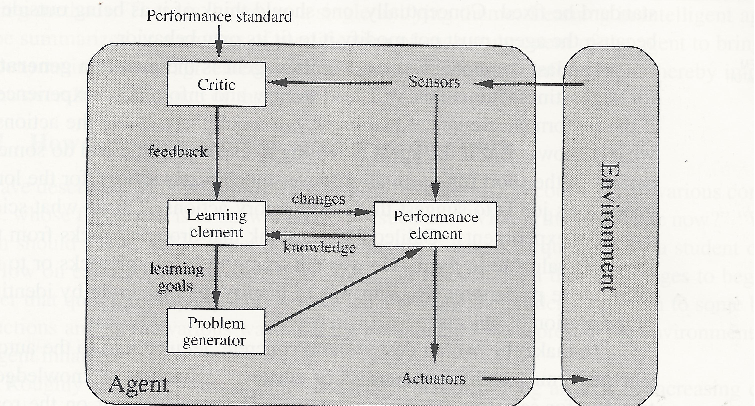
\includegraphics[height =.6\textheight,width=.7\textwidth]{figuras/agent-learning.pdf}
\caption{Arquitetura agente com aprendizagem}
\label{ag_01}
\end{figure}
    
\end{frame}

